%-*-latex-*-
\mychapter{103}{4800}{Distribution sort}

\newpage%-*-latex-*-
\sectionthree{Distribution sort: counting sort}
\begin{python0}
from solutions import *; clear()
\end{python0}

Beside sorting an array using a comparison-based sorting
algorithm, i.e., using $\leq$ or $<$ or $\geq$ or $>$ to compare values in the array,
there's
another class of sorting algorithms that work in a difference way.
Distribution sorting algoroithms sort by \textit{distributing}
the values in an array.
Sometimes distribution sort will use a comparison-based sort.

The simplest distribution sort is the counting sort.

Suppose you have an array \verb!x! of integers with values
from 0 to 4 (inclusive):

%-*-latex-*-
{\footnotesize \begin{Verbatim}[frame=single,fontsize=\small]
[student@localhost discrete-probability] python tossfaircoin1.py
experiment 0 ... outcome: HEAD
experiment 1 ... outcome: TAIL
experiment 2 ... outcome: HEAD
experiment 3 ... outcome: TAIL
experiment 4 ... outcome: HEAD
experiment 5 ... outcome: TAIL
experiment 6 ... outcome: TAIL
experiment 7 ... outcome: TAIL
experiment 8 ... outcome: TAIL
experiment 9 ... outcome: TAIL
experiment 10 ... outcome: TAIL
experiment 11 ... outcome: HEAD
experiment 12 ... outcome: HEAD
experiment 13 ... outcome: TAIL
experiment 14 ... outcome: HEAD
experiment 15 ... outcome: HEAD
experiment 16 ... outcome: HEAD
experiment 17 ... outcome: TAIL
experiment 18 ... outcome: TAIL
experiment 19 ... outcome: HEAD
\end{Verbatim}
}


You scan the array and count the number of times each value
from 0 to 4 occurs in \verb!x!.

\begin{center}
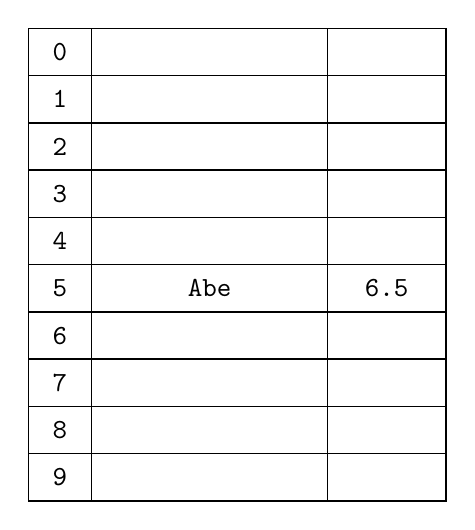
\begin{tikzpicture}

\draw (1.4, 0.7)
  node[draw, line width=0.02cm, , color=black,
       rounded corners=0cm, inner sep=0cm] {

\begin{minipage}[t][0.6cm]{0.8cm}
\mbox{}

\end{minipage}

};\draw (1.4, 0.7) node[color=black] {{\texttt{0}}};
\draw (3.3, 0.7)
  node[draw, line width=0.02cm, , color=black,
       rounded corners=0cm, inner sep=0cm] {

\begin{minipage}[t][0.6cm]{3.0cm}
\mbox{}

\end{minipage}

};\draw (3.3, 0.7) node[color=black] {{\texttt{}}};
\draw (5.55, 0.7)
  node[draw, line width=0.02cm, , color=black,
       rounded corners=0cm, inner sep=0cm] {

\begin{minipage}[t][0.6cm]{1.5cm}
\mbox{}

\end{minipage}

};\draw (5.55, 0.7) node[color=black] {{\texttt{}}};
\draw (1.4, 0.09999999999999987)
  node[draw, line width=0.02cm, , color=black,
       rounded corners=0cm, inner sep=0cm] {

\begin{minipage}[t][0.6cm]{0.8cm}
\mbox{}

\end{minipage}

};\draw (1.4, 0.09999999999999987) node[color=black] {{\texttt{1}}};
\draw (3.3, 0.09999999999999987)
  node[draw, line width=0.02cm, , color=black,
       rounded corners=0cm, inner sep=0cm] {

\begin{minipage}[t][0.6cm]{3.0cm}
\mbox{}

\end{minipage}

};\draw (3.3, 0.09999999999999987) node[color=black] {{\texttt{}}};
\draw (5.55, 0.09999999999999987)
  node[draw, line width=0.02cm, , color=black,
       rounded corners=0cm, inner sep=0cm] {

\begin{minipage}[t][0.6cm]{1.5cm}
\mbox{}

\end{minipage}

};\draw (5.55, 0.09999999999999987) node[color=black] {{\texttt{}}};
\draw (1.4, -0.5000000000000002)
  node[draw, line width=0.02cm, , color=black,
       rounded corners=0cm, inner sep=0cm] {

\begin{minipage}[t][0.6cm]{0.8cm}
\mbox{}

\end{minipage}

};\draw (1.4, -0.5000000000000002) node[color=black] {{\texttt{2}}};
\draw (3.3, -0.5000000000000002)
  node[draw, line width=0.02cm, , color=black,
       rounded corners=0cm, inner sep=0cm] {

\begin{minipage}[t][0.6cm]{3.0cm}
\mbox{}

\end{minipage}

};\draw (3.3, -0.5000000000000002) node[color=black] {{\texttt{}}};
\draw (5.55, -0.5000000000000002)
  node[draw, line width=0.02cm, , color=black,
       rounded corners=0cm, inner sep=0cm] {

\begin{minipage}[t][0.6cm]{1.5cm}
\mbox{}

\end{minipage}

};\draw (5.55, -0.5000000000000002) node[color=black] {{\texttt{}}};
\draw (1.4, -1.1000000000000003)
  node[draw, line width=0.02cm, , color=black,
       rounded corners=0cm, inner sep=0cm] {

\begin{minipage}[t][0.6cm]{0.8cm}
\mbox{}

\end{minipage}

};\draw (1.4, -1.1000000000000003) node[color=black] {{\texttt{3}}};
\draw (3.3, -1.1000000000000003)
  node[draw, line width=0.02cm, , color=black,
       rounded corners=0cm, inner sep=0cm] {

\begin{minipage}[t][0.6cm]{3.0cm}
\mbox{}

\end{minipage}

};\draw (3.3, -1.1000000000000003) node[color=black] {{\texttt{}}};
\draw (5.55, -1.1000000000000003)
  node[draw, line width=0.02cm, , color=black,
       rounded corners=0cm, inner sep=0cm] {

\begin{minipage}[t][0.6cm]{1.5cm}
\mbox{}

\end{minipage}

};\draw (5.55, -1.1000000000000003) node[color=black] {{\texttt{}}};
\draw (1.4, -1.7000000000000002)
  node[draw, line width=0.02cm, , color=black,
       rounded corners=0cm, inner sep=0cm] {

\begin{minipage}[t][0.6cm]{0.8cm}
\mbox{}

\end{minipage}

};\draw (1.4, -1.7000000000000002) node[color=black] {{\texttt{4}}};
\draw (3.3, -1.7000000000000002)
  node[draw, line width=0.02cm, , color=black,
       rounded corners=0cm, inner sep=0cm] {

\begin{minipage}[t][0.6cm]{3.0cm}
\mbox{}

\end{minipage}

};\draw (3.3, -1.7000000000000002) node[color=black] {{\texttt{}}};
\draw (5.55, -1.7000000000000002)
  node[draw, line width=0.02cm, , color=black,
       rounded corners=0cm, inner sep=0cm] {

\begin{minipage}[t][0.6cm]{1.5cm}
\mbox{}

\end{minipage}

};\draw (5.55, -1.7000000000000002) node[color=black] {{\texttt{}}};
\draw (1.4, -2.3000000000000003)
  node[draw, line width=0.02cm, , color=black,
       rounded corners=0cm, inner sep=0cm] {

\begin{minipage}[t][0.6cm]{0.8cm}
\mbox{}

\end{minipage}

};\draw (1.4, -2.3000000000000003) node[color=black] {{\texttt{5}}};
\draw (3.3, -2.3000000000000003)
  node[draw, line width=0.02cm, , color=black,
       rounded corners=0cm, inner sep=0cm] {

\begin{minipage}[t][0.6cm]{3.0cm}
\mbox{}

\end{minipage}

};\draw (3.3, -2.3000000000000003) node[color=black] {{\texttt{Abe}}};
\draw (5.55, -2.3000000000000003)
  node[draw, line width=0.02cm, , color=black,
       rounded corners=0cm, inner sep=0cm] {

\begin{minipage}[t][0.6cm]{1.5cm}
\mbox{}

\end{minipage}

};\draw (5.55, -2.3000000000000003) node[color=black] {{\texttt{6.5}}};
\draw (1.4, -2.9000000000000004)
  node[draw, line width=0.02cm, , color=black,
       rounded corners=0cm, inner sep=0cm] {

\begin{minipage}[t][0.6cm]{0.8cm}
\mbox{}

\end{minipage}

};\draw (1.4, -2.9000000000000004) node[color=black] {{\texttt{6}}};
\draw (3.3, -2.9000000000000004)
  node[draw, line width=0.02cm, , color=black,
       rounded corners=0cm, inner sep=0cm] {

\begin{minipage}[t][0.6cm]{3.0cm}
\mbox{}

\end{minipage}

};\draw (3.3, -2.9000000000000004) node[color=black] {{\texttt{}}};
\draw (5.55, -2.9000000000000004)
  node[draw, line width=0.02cm, , color=black,
       rounded corners=0cm, inner sep=0cm] {

\begin{minipage}[t][0.6cm]{1.5cm}
\mbox{}

\end{minipage}

};\draw (5.55, -2.9000000000000004) node[color=black] {{\texttt{}}};
\draw (1.4, -3.500000000000001)
  node[draw, line width=0.02cm, , color=black,
       rounded corners=0cm, inner sep=0cm] {

\begin{minipage}[t][0.6cm]{0.8cm}
\mbox{}

\end{minipage}

};\draw (1.4, -3.500000000000001) node[color=black] {{\texttt{7}}};
\draw (3.3, -3.500000000000001)
  node[draw, line width=0.02cm, , color=black,
       rounded corners=0cm, inner sep=0cm] {

\begin{minipage}[t][0.6cm]{3.0cm}
\mbox{}

\end{minipage}

};\draw (3.3, -3.500000000000001) node[color=black] {{\texttt{}}};
\draw (5.55, -3.500000000000001)
  node[draw, line width=0.02cm, , color=black,
       rounded corners=0cm, inner sep=0cm] {

\begin{minipage}[t][0.6cm]{1.5cm}
\mbox{}

\end{minipage}

};\draw (5.55, -3.500000000000001) node[color=black] {{\texttt{}}};
\draw (1.4, -4.1000000000000005)
  node[draw, line width=0.02cm, , color=black,
       rounded corners=0cm, inner sep=0cm] {

\begin{minipage}[t][0.6cm]{0.8cm}
\mbox{}

\end{minipage}

};\draw (1.4, -4.1000000000000005) node[color=black] {{\texttt{8}}};
\draw (3.3, -4.1000000000000005)
  node[draw, line width=0.02cm, , color=black,
       rounded corners=0cm, inner sep=0cm] {

\begin{minipage}[t][0.6cm]{3.0cm}
\mbox{}

\end{minipage}

};\draw (3.3, -4.1000000000000005) node[color=black] {{\texttt{}}};
\draw (5.55, -4.1000000000000005)
  node[draw, line width=0.02cm, , color=black,
       rounded corners=0cm, inner sep=0cm] {

\begin{minipage}[t][0.6cm]{1.5cm}
\mbox{}

\end{minipage}

};\draw (5.55, -4.1000000000000005) node[color=black] {{\texttt{}}};
\draw (1.4, -4.7)
  node[draw, line width=0.02cm, , color=black,
       rounded corners=0cm, inner sep=0cm] {

\begin{minipage}[t][0.6cm]{0.8cm}
\mbox{}

\end{minipage}

};\draw (1.4, -4.7) node[color=black] {{\texttt{9}}};
\draw (3.3, -4.7)
  node[draw, line width=0.02cm, , color=black,
       rounded corners=0cm, inner sep=0cm] {

\begin{minipage}[t][0.6cm]{3.0cm}
\mbox{}

\end{minipage}

};\draw (3.3, -4.7) node[color=black] {{\texttt{}}};
\draw (5.55, -4.7)
  node[draw, line width=0.02cm, , color=black,
       rounded corners=0cm, inner sep=0cm] {

\begin{minipage}[t][0.6cm]{1.5cm}
\mbox{}

\end{minipage}

};\draw (5.55, -4.7) node[color=black] {{\texttt{}}};
\end{tikzpicture}

\end{center}



For instance \verb!count[2]! is the number of times \verb!2!
occurs in array \verb!x!.

Now the final thing to do is to fill \verb!x! using
information in \verb!count!.
For instance \verb!count[0]! is \verb!2!, 
so I would put two \verb!0!'s into \verb!x!:

\begin{center}
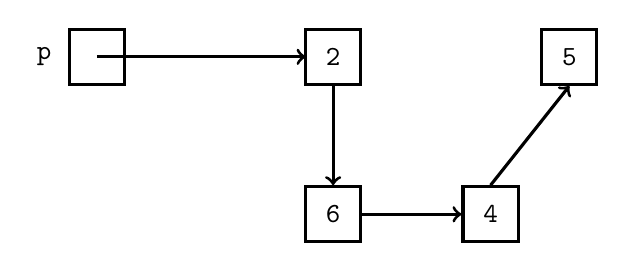
\begin{tikzpicture}

\draw (0.35, 0.35)
  node[draw, line width=0.04cm, , color=black,
       rounded corners=0cm, inner sep=0cm] {

\begin{minipage}[t][0.7cm]{0.7cm}
\mbox{}

\end{minipage}

};\draw (0.35, 0.35) node[color=black] {{\texttt{2}}};
\draw (0.35, -1.65)
  node[draw, line width=0.04cm, , color=black,
       rounded corners=0cm, inner sep=0cm] {

\begin{minipage}[t][0.7cm]{0.7cm}
\mbox{}

\end{minipage}

};\draw (0.35, -1.65) node[color=black] {{\texttt{6}}};
\draw (2.35, -1.65)
  node[draw, line width=0.04cm, , color=black,
       rounded corners=0cm, inner sep=0cm] {

\begin{minipage}[t][0.7cm]{0.7cm}
\mbox{}

\end{minipage}

};\draw (2.35, -1.65) node[color=black] {{\texttt{4}}};
\draw (3.35, 0.35)
  node[draw, line width=0.04cm, , color=black,
       rounded corners=0cm, inner sep=0cm] {

\begin{minipage}[t][0.7cm]{0.7cm}
\mbox{}

\end{minipage}

};\draw (3.35, 0.35) node[color=black] {{\texttt{5}}};\draw[line width=0.04cm,black,->] (0.35,-0.02) to  (0.35,-1.28);
\draw[line width=0.04cm,black,->] (0.72,-1.65) to  (1.98,-1.65);
\draw[line width=0.04cm,black,->] (2.35,-1.28) to  (3.35,-0.02);

\draw (-2.65, 0.35)
  node[draw, line width=0.04cm, , color=black,
       rounded corners=0cm, inner sep=0cm] {

\begin{minipage}[t][0.7cm]{0.7cm}
\mbox{}

\end{minipage}

};\draw (-2.65, 0.35) node[color=black] {{\texttt{}}};\draw[line width=0.04cm,black,->] (-2.65,0.35) to  (0,0.35);

\draw (-3.32, 0.35)
  node[draw, line width=0.04cm, , color=white,
       rounded corners=0cm, inner sep=0cm] {

\begin{minipage}[t][0.1cm]{0.1cm}
\mbox{}

\end{minipage}

};\draw (-3.32, 0.35) node[color=black] {{\texttt{p}}};
\end{tikzpicture}

\end{center}



Next, since \verb!count[1]! is \verb!0!, \verb!1! does not appear in 
\verb!x!.
So the re-organized \verb!x! looks like this (i.e., no change):

\begin{center}
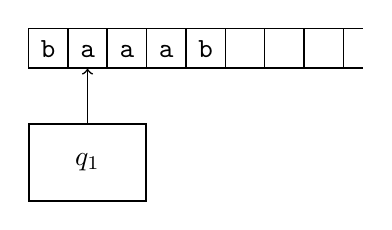
\begin{tikzpicture}

\draw (0.25, 0.25)
  node[draw, line width=0.02cm, , color=black,
       rounded corners=0cm, inner sep=0cm] {

\begin{minipage}[t][0.5cm]{0.5cm}
\mbox{}

\end{minipage}

};\draw (0.25, 0.25) node[color=black] {{\vphantom{baaab\SPACE\SPACE\SPACE}\texttt{b}}};
\draw (0.75, 0.25)
  node[draw, line width=0.02cm, , color=black,
       rounded corners=0cm, inner sep=0cm] {

\begin{minipage}[t][0.5cm]{0.5cm}
\mbox{}

\end{minipage}

};\draw (0.75, 0.25) node[color=black] {{\vphantom{baaab\SPACE\SPACE\SPACE}\texttt{a}}};
\draw (1.25, 0.25)
  node[draw, line width=0.02cm, , color=black,
       rounded corners=0cm, inner sep=0cm] {

\begin{minipage}[t][0.5cm]{0.5cm}
\mbox{}

\end{minipage}

};\draw (1.25, 0.25) node[color=black] {{\vphantom{baaab\SPACE\SPACE\SPACE}\texttt{a}}};
\draw (1.75, 0.25)
  node[draw, line width=0.02cm, , color=black,
       rounded corners=0cm, inner sep=0cm] {

\begin{minipage}[t][0.5cm]{0.5cm}
\mbox{}

\end{minipage}

};\draw (1.75, 0.25) node[color=black] {{\vphantom{baaab\SPACE\SPACE\SPACE}\texttt{a}}};
\draw (2.25, 0.25)
  node[draw, line width=0.02cm, , color=black,
       rounded corners=0cm, inner sep=0cm] {

\begin{minipage}[t][0.5cm]{0.5cm}
\mbox{}

\end{minipage}

};\draw (2.25, 0.25) node[color=black] {{\vphantom{baaab\SPACE\SPACE\SPACE}\texttt{b}}};
\draw (2.75, 0.25)
  node[draw, line width=0.02cm, , color=black,
       rounded corners=0cm, inner sep=0cm] {

\begin{minipage}[t][0.5cm]{0.5cm}
\mbox{}

\end{minipage}

};\draw (2.75, 0.25) node[color=black] {{\vphantom{baaab\SPACE\SPACE\SPACE}\texttt{\SPACE}}};
\draw (3.25, 0.25)
  node[draw, line width=0.02cm, , color=black,
       rounded corners=0cm, inner sep=0cm] {

\begin{minipage}[t][0.5cm]{0.5cm}
\mbox{}

\end{minipage}

};\draw (3.25, 0.25) node[color=black] {{\vphantom{baaab\SPACE\SPACE\SPACE}\texttt{\SPACE}}};
\draw (3.75, 0.25)
  node[draw, line width=0.02cm, , color=black,
       rounded corners=0cm, inner sep=0cm] {

\begin{minipage}[t][0.5cm]{0.5cm}
\mbox{}

\end{minipage}

};\draw (3.75, 0.25) node[color=black] {{\vphantom{baaab\SPACE\SPACE\SPACE}\texttt{\SPACE}}};\draw[line width=0.02cm,black] (4.0,0.5) to  (4.25,0.5);
\draw[line width=0.02cm,black] (4.0,0.0) to  (4.25,0.0);

\draw (0.75, -1.2)
  node[draw, line width=0.02cm, , color=black,
       rounded corners=0cm, inner sep=0cm] {

\begin{minipage}[t][0.98cm]{1.48cm}
\mbox{}

\end{minipage}

};\draw (0.75, -1.2) node[color=black] {$q_1$};\draw[line width=0.02cm,black,->] (0.75,-0.7) to  (0.75,-0.47) to  (0.75,-0.47) to  (0.75,-0.01);
\end{tikzpicture}

\end{center}



However note that \verb!count[2]! is \verb!3!, which means that
\verb!2! appears \verb!3! times.
Therefore my \verb!x! now look like this:

\begin{center}
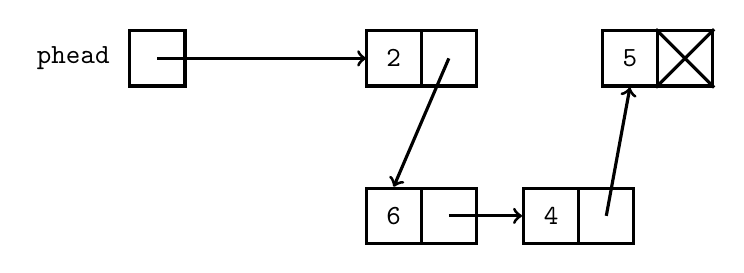
\begin{tikzpicture}

\draw (0.35, 0.35)
  node[draw, line width=0.04cm, , color=black,
       rounded corners=0cm, inner sep=0cm] {

\begin{minipage}[t][0.7cm]{0.7cm}
\mbox{}

\end{minipage}

};\draw (0.35, 0.35) node[color=black] {{\texttt{2}}};
\draw (1.0499999999999998, 0.35)
  node[draw, line width=0.04cm, , color=black,
       rounded corners=0cm, inner sep=0cm] {

\begin{minipage}[t][0.7cm]{0.7cm}
\mbox{}

\end{minipage}

};\draw (1.0499999999999998, 0.35) node[color=black] {{\texttt{}}};
\draw (0.35, -1.65)
  node[draw, line width=0.04cm, , color=black,
       rounded corners=0cm, inner sep=0cm] {

\begin{minipage}[t][0.7cm]{0.7cm}
\mbox{}

\end{minipage}

};\draw (0.35, -1.65) node[color=black] {{\texttt{6}}};
\draw (1.0499999999999998, -1.65)
  node[draw, line width=0.04cm, , color=black,
       rounded corners=0cm, inner sep=0cm] {

\begin{minipage}[t][0.7cm]{0.7cm}
\mbox{}

\end{minipage}

};\draw (1.0499999999999998, -1.65) node[color=black] {{\texttt{}}};
\draw (2.35, -1.65)
  node[draw, line width=0.04cm, , color=black,
       rounded corners=0cm, inner sep=0cm] {

\begin{minipage}[t][0.7cm]{0.7cm}
\mbox{}

\end{minipage}

};\draw (2.35, -1.65) node[color=black] {{\texttt{4}}};
\draw (3.0500000000000003, -1.65)
  node[draw, line width=0.04cm, , color=black,
       rounded corners=0cm, inner sep=0cm] {

\begin{minipage}[t][0.7cm]{0.7cm}
\mbox{}

\end{minipage}

};\draw (3.0500000000000003, -1.65) node[color=black] {{\texttt{}}};
\draw (3.35, 0.35)
  node[draw, line width=0.04cm, , color=black,
       rounded corners=0cm, inner sep=0cm] {

\begin{minipage}[t][0.7cm]{0.7cm}
\mbox{}

\end{minipage}

};\draw (3.35, 0.35) node[color=black] {{\texttt{5}}};
\draw (4.05, 0.35)
  node[draw, line width=0.04cm, , color=black,
       rounded corners=0cm, inner sep=0cm] {

\begin{minipage}[t][0.7cm]{0.7cm}
\mbox{}

\end{minipage}

};\draw (4.05, 0.35) node[color=black] {{\texttt{}}};\draw[line width=0.04cm,black,->] (1.05,0.35) to  (0.35,-1.28);
\draw[line width=0.04cm,black,->] (1.05,-1.65) to  (1.98,-1.65);
\draw[line width=0.04cm,black,->] (3.05,-1.65) to  (3.35,-0.02);
\draw[line width=0.04cm,black] (3.68,0.72) to  (4.42,-0.02);
\draw[line width=0.04cm,black] (4.42,0.72) to  (3.68,-0.02);

\draw (-2.65, 0.35)
  node[draw, line width=0.04cm, , color=black,
       rounded corners=0cm, inner sep=0cm] {

\begin{minipage}[t][0.7cm]{0.7cm}
\mbox{}

\end{minipage}

};\draw (-2.65, 0.35) node[color=black] {{\texttt{}}};\draw[line width=0.04cm,black,->] (-2.65,0.35) to  (0,0.35);

\draw (-3.7199999999999998, 0.35)
  node[draw, line width=0.04cm, , color=white,
       rounded corners=0cm, inner sep=0cm] {

\begin{minipage}[t][0.1cm]{0.1cm}
\mbox{}

\end{minipage}

};\draw (-3.7199999999999998, 0.35) node[color=black] {{\texttt{phead}}};
\end{tikzpicture}

\end{center}



You get the point.

The pseudocode looks like this.
I assume that the values in \verb!x! are from 0 to \verb!M!.
\begin{console}
ALGORITHM: counting_sort
INPUT: array x of size n

    count = int array of size M + 1, initialized with 0s
    for i = 0, 1, 2, ..., n - 1:
        count[x[i]] = count[x[i]] + 1
    j = 0
    for i = 0, 1, 2, ..., M:
        for k = 1, ..., count[i]:
            x[j] = i
            j = j + 1
\end{console}

If \verb!M! is not 
known, you have to run through \verb!x! to figure that out.


Here's the runtime analysis.
The time to create \verb!count!, if it's in the heap,
might very well be $O(1)$ (or the memory allocation might fail because of lack of
available memory). So that's hard to say.
So let's just assume memory allocation for \verb!count! is negligible.
First you have to set the \verb!count! array to zeroes:
that takes $A(M + 1)$ ($A$ is a constant).
You need to run through \verb!x! to fill \verb!count! with
values: that takes a time of $Bn$.
You will to put values back into \verb!x! using \verb!count!.
That requires touching each cell in \verb!x!.
So for this part, the runtime is $Cn$.
Altogether, the runtime is
\[
O(n + M)
\]
Of course the space requirement is
\[
O(M + 1) = O(M)
\]

\newpage

\begin{ex}
  How would you sort a huge array if the values are integer in the interval $[-10, 10]$?
  \qed
\end{ex}


\begin{ex}
  How would you sort a huge array if the values are
  1000000, 1100000, 1200000, 1300000, ..., 1900000.
  \qed
\end{ex}


\begin{ex}
  Modify the counting sort algorithm to sort a huge array of \verb!double!s
  where there is a (known) small number of distinct \verb!double! values in the 
  array.
  Say the size of the array is $10^6$ and there are at most $1000$ distinct
  \verb!double!s in the array.
  What if the values are not known ahead of time?
  (The idea should also work for other types.)
  \qed
\end{ex}


\begin{ex}
Take a look at the sieve of Eratosthenes and you'll see that it's related to 
the counting sort.
\qed
\end{ex}

\newpage%-*-latex-*-
\section{LSD radix sort}

There are two basic variants of radix sort.
First I'll talk about the LSD (least significant digit) radix sort.


Suppose you have the following array (I'm going to draw it vertically):
\begin{python}
from latextool_basic import *
p = Plot()

def arr(x=0, y=0, xs=[]):
    xs = [[_] for _ in xs]
    return Array2d(x, y, xs, width=0.7, height=0.7)

def string(x=0, y=0, label=''):
    label = r'\text{\texttt{%s}}' % label
    return Rect2(x, y, x, y, label=label, linewidth=0)

a = arr(xs=[31,22,'02',25,34,41,'09'])
p += a
x, y = a[0][0].left()
p += string(x-0.3, y, 'x')
print(p)
\end{python}
First we sort the array \textit{by the ones digit} using a 
\textit{stable} sorting algorithm (example: mergesort).
\begin{python}
from latextool_basic import *
p = Plot()

def arr(x=0, y=0, xs=[]):
    xs = [[_] for _ in xs]
    return Array2d(x, y, xs, width=0.7, height=0.7)

def string(x=0, y=0, label=''):
    label = r'\text{\texttt{%s}}' % label
    return Rect2(x, y, x, y, label=label, linewidth=0)

def bubble(xs, f):
    n = len(xs)
    #print "xs:", xs
    for i in range(n - 2, -1, -1):
        for j in range(0, i + 1):
            if f(xs[j]) > f(xs[j + 1]):
                xs[j], xs[j + 1] = xs[j + 1], xs[j]
        #print "xs:", xs

a = ['31','22','02','25','34','41','09']
a = [(_[-1],_) for _ in a]
bubble(a, lambda x:x[0])
a = [_ for __,_ in a] 
a = arr(xs=a)
p += a
x, y = a[0][0].left()
p += string(x-0.3, y, 'x')
print(p)
\end{python}
Because the sorting is stable, note for instance that 
\verb!22! appear before \verb!02! before and after the sort.

Next I'm going to perform a stable sort on the tens digit:
\begin{python}
from latextool_basic import *
p = Plot()

def arr(x=0, y=0, xs=[]):
    xs = [[_] for _ in xs]
    return Array2d(x, y, xs, width=0.7, height=0.7)

def string(x=0, y=0, label=''):
    label = r'\text{\texttt{%s}}' % label
    return Rect2(x, y, x, y, label=label, linewidth=0)

def bubble(xs, f):
    n = len(xs)
    #print "xs:", xs
    for i in range(n - 2, -1, -1):
        for j in range(0, i + 1):
            if f(xs[j]) > f(xs[j + 1]):
                xs[j], xs[j + 1] = xs[j + 1], xs[j]
        #print "xs:", xs

a = ['31','22','02','25','34','41','09']
a = [(_[-1],_) for _ in a]
bubble(a, lambda x:x[0])
bubble(a, lambda x:x[1])
a = [_ for __,_ in a] 
a = arr(xs=a)
p += a
x, y = a[0][0].left()
p += string(x-0.3, y, 'x')
print(p)
\end{python}

Note for each pass of the radix sort, you can use any stable sort.
You want to pick the fastest (of course): so of course mergesort is better than bubblesort!
If you are using mergesort to sort the ones and then the tens, then the
runtime is
\[
  O(2 n \lg n) = O(n \lg n)
\]
If there are $d$ digits (instead of $2$), then the runtime is
\[
  O(d n \lg n)
\]
If most cases, the $d$ might be a constant (i.e., does not change).
For instance if your array is an array of integers in a 32-bit
computer, then $d = 10$.
In this case the runtime is
\[
  O(d n \lg n) = O(n \ln n)
\]

For radix sort, when you look at the key \verb!31! (the first value of the
original array) and you are sorting based on the first digit of \verb!31!,
i.e., \verb!1!, we say that \verb!1! is the \defone{subkey}.
If there's no digit there, for instance look at the key \verb!02! which is
actually \verb!2!, then the second digit subkey of \verb!2! = \verb!02! is
\verb!0!, i.e., the smallest possible subkey value (if you sorting in
ascending order). 

For implementation, you might want to have a \verb!subkey! function.
\verb!subkey(key, i)! returns the $i$--th digit of \verb!key! where
$i$ starts with $0$ (the leftmost digit).
If you call \verb!subkey(31, 0)!, you get \verb!1!.
If you call \verb!subkey(31, 1)!, you get \verb!3!.
Remember that since \verb!2! has only one digit,
if you call \verb!subkey(2, 1)!, you get \verb!0!.

There's another way to do this with a better runtime.

Recall the concept of a queue, a data structure there data enters at
the tail of the data structure and leave through the head of the data structure:

\begin{python}
from latextool_basic import *
from latexcircuit import *
p = Plot()
r = Rect(x0=0, y0=0, x1=5, y1=0.8)
p += r

x,y = r.right()
p += Line(points=[(x+2,y), (x+0.2,y)], endstyle='>', linewidth=0.1)

x,y = r.left()
p += Line(points=[(x-0.2,y), (x - 2,y)], endstyle='>', linewidth=0.1)

x,y = r.bottomleft()
X = POINT(x=x, y=y, r=0, label='head', anchor='north west')
p += str(X)

x,y = r.bottomright()
X = POINT(x=x, y=y, r=0, label='tail', anchor='north east')
p += str(X)

print(p)
\end{python}

We saw the queue in CISS245 where we implemented it using an array
(say dynamic arrays in the heap).
The worst runtimes are insert and delete are
\begin{tightlist}
\item entering the queue: $T(n) = O(n)$  
\item leaving the queue: $T(n) = O(n)$ 
\end{tightlist}
where $n$ is the size of the queue.

There's a better way to implement a queue ...

After we study linked list, you will see that you can implement a queue using
linked lists.
The operations 
on a queue implemented using a linked list has the following runtimes:
\begin{tightlist}
\item entering the queue: $T(n) = O(1)$ 
\item leaving the queue: $T(n) = O(1)$ 
\end{tightlist}
where $n$ is the size of the queue.

We then sort based on the digit value in the following way:
First we create an array \verb!q! of 10 queues.
\verb!q[0]! is a queue that will hold values with digit value of \verb!0!,
\verb!q[1]! is a queue that will hold values with digit value of \verb!1!, etc.
For each value of \verb!x!, we place the value into the appropriate queue
based on the digit of that value.
When we're done, we remove all the values in \verb!q[0]! and place them
in order into \verb!x!.
We then repeat with \verb!q[1]!, etc.
Because the operations on the queue all have runtime of $O(1)$,
the total runtime is $O(n)$.

We then repeat the process, but now determine which queue a value of \verb!x!
should go into by the tens digit of that value.
Altogether the runtime is $O(2n)$.

In our example above, the numbers have 2 digits.
If the numbers have $d$ digits, then the runtime is $O(dn)$.
If the number of digits $d$ is fixed (i.e., is a constant),
then the runtime is $O(n)$.

For space, the total amount of memory used by the queues 
adds up to 
$O(n)$.
So although the queue-based version of radix sort is faster,
it's at the expense of memory.
Remember that.
Nothing is for free.

Note that by using queues, 
the sorting process is stable:
a number that has joined a queue will always be ahead of another
that joined the queue later.
After each pass, the values of a queues are dequeued and put back 
into the original array, of course starting with 
the queue corresonding to \verb!0!.

Note that when we use queues for distribution, a value
enters the queue without being compared when other values.
Therefore in this context radix sort is a distribution (non-comparison) sorting
algorithm.

Another thing to note is that we are assuming all the numbers
we are sorting have the same number of digits.
What if the number of digits are different?
As mentioned above, if you call \verb!subkey(key, i)!
and \verb!key! has no digit at \verb!i!,
\verb!subkey(key, i)! returns the smallest possible digit value, i.e., \verb!0!.

The above starts with the \lq\lq smallest" digit (i.e., the ones digit).
That's why it's called \defone{least signicant digit (LSD) radix sort}.

\newpage

\begin{ex}
  Perform LSD radix sort on the following values, showing the
  values of the array after each pass:
  \[
    121, 23, 231, 89, 123, 536, 697, 457, 355, 243, 657, 345, 174, 248, 346, 376
  \]
  \qed
\end{ex}

\begin{ex}
What happens when you sort not by single digit for each pass, but
\textit{two} digits?
\qed
\end{ex}



\newpage
\section{MSD radix sort}

Instead of sorting numbers by sorting on their digits from right to left, i.e.,
starting with the least significant digit,
you can do the same thing but going left to right.
That's \defone{MSD radix sort} (MSD = most significant digit).
If you
sort numbers using MSD
radix sort on
\[
22, 19, 31, 91, 90, 10, 45
\]
after the first pass (i.e., after stable sorting on the tens), you 
you will see this:
\[
19, 10, 22, 31, 45, 91, 90
\]
Now we (stable) sort by the ones:
\[
10, 90, 31, 91, 22, 45, 19
\]




For numbers with different lengths, you can
pad on the right with an extra \lq\lq digit'' that is infinitely small.
For instance, say you pad the above on the right with \verb!?!
and assume that $? < 0 < 1 < 2 < 3 < 4 < 5 < 6 < 7 < 8 < 9$ to get
\[
2?, 1?, 3?, 91, 9?, 19, 45
\]
Then after performing a stable sorting on the leftmost digit, I get
\[
1?, 19, 2?, 3?, 45, 91, 9?, 
\]
and on after the second pass of stable sorting on the second digit, I get
\[
1?, 19, 2?, 3?, 45, 9?, 91  
\]
After the array is sorted, you can remove this extra data \verb!?! to get
\[
1, 19, 2, 3, 45, 9, 91  
\]

If you think that's bizarre, then think again -- you have
seen this before.
Let's look at strings.
Suppose you have an array of string
\verb!"apple"!,
\verb!"abe"!,
\verb!"cat"!,
\verb!"ab"!,
\verb!"bee"!,
\verb!"cap"!.
Using MSD radix sort, you would get
\[
\texttt{"ab",
"abe",
"apple",
"bee",
"cap".
"cat"}
\]
where the order of each character is determined by its ASCII code.

The above ordering is called \defterm{dictionary order}. Duh.

Note that you  don't really need to \lq\lq pad on the right''.
For instance when comparing strings using the dictionary ordering
on C-strings $x$ and $y$ to compute the boolean value of
$x < y$,
you run a loop comparing \verb!x[i]! and \verb!y[i]!.
If \verb!i! is less than the length of \verb!x! but $\geq$ the length of
\verb!y!,
you return true.
If \verb!i! is less than the length of \verb!y! but $\geq$ the length of
\verb!x!,
you return false.
If \verb!x[i]! $<$ \verb!y[i]!, you return true.
If \verb!x[i]! $>$ \verb!y[i]!, you return false.
If \verb!x[i]! \verb!==! \verb!y[i]!, you increment \verb!i! and
continue on to the next iteration of the loop.

\newpage%-*-latex-*-
\sectionthree{Bucket sort}
\begin{python0}
from solutions import *; clear()
\end{python0}

The bucket sort is very similar to the radix sort.

Recall that when I was talking about the radix sort, I use
10 linked lists as queues to sort integers in each pass of the radix sort.
I'm going to do it again, but in a different way.

It's really pretty easy.
Suppose I know that my arrays always have values from 0 to 99.
Then I can create 10 bucket.
I scan the array and if a value of the element
has value from 0 to 9, I put it into bucket 0.
If the value is from 10 to 19, I put it into bucket has 1. 
Etc.
If the number of values is a bucket is small,
I can use any suitable sorting algorithm to sort values in the bucket.
If there are too many values, of course I can use a suitable 
sorting algorithm, including the bucket sorting algorithm,
So suppose for my first bucket that holds values 0 to 9, I have 1000.
Since there are only 10 possible values, I would choose the counting sort
and sort the bucket. 
That's it.

But what if the values are from 0 to 999999999?
I can have have 10 buckets again and if the 
range of values of the buckets are the same, then
the first bucket would hold values from 0 to 99999999.
Unfortunately, it might not be a good idea to use the counting sort.
You have to decide on what other sorting algorithm to use.
If you use bucket sort again, then, of course each bucket this
time will have a smaller range of values.
If you do this recursively, of course, at some point, the number of
values in a bucket will shrink -- except for the case when there's clustering,
i.e., there are lots of values clustered
together.

Assume the values are uniformly distributed
and you want to minimize memory usage, you can use a linked list (see chapter
on linked list) for each bucket.
The space complexity is minimal when compared to using vectors.
Note that insertion sort can be performed on linked lists (the buckets in
this case).
Then the values from the buckets can be copied back to the original input
array.
If $n$ linked list are used and the keys are uniformly distributed
over an interval $[a, b]$, then each buckey can be used to collect
keys in a subinterval or length $(b - a)/n$.



\begin{comment}
Suppose you have an array of size 5 which is a permutation of 0..4, say
\verb!x = [3,2,1,0]!.
For each $i = 0, 1, 2, 3$, put $x[i]$ into its right place by
swapping it with the value occupying where $x[i]$ should be.
For instance $x[0] = 3$, so $x[0]$ should go into index 3 location.
Therefore you swap $x[0]$ and $x[3]$.
This gives you
\verb!x = [0,2,1,3]!.
For index $ = 1$, you get this:
\verb!x = [0,1,2,3]!.
For $i = 2$, there's no change.
For $i = 3$, there's no change.
\end{comment}

\begin{python0}
from solutions import *
prepare_solutions()
\end{python0}

\newpage
\section*{Solutions}
Solution to Exercise \ref{ex:power-series-11}\labeltext{}{sol:power-series-11}.

\debug{\tinysidebar{exercises/{power-series-11/answer.tex}}}
 
(a) From
\begin{align*}
\sum_{n = 0}^\infty \frac{1}{2^n} x^n \cdot \sum_{n = 0}^\infty \frac{1}{2^n} x^n
&=
\left(
1 + \frac{1}{2}x + \frac{1}{4}x^2 + \frac{1}{8}x^3 + \cdots
\right)
\left(
1 + \frac{1}{2}x + \frac{1}{4}x^2 + \frac{1}{8}x^3 + \cdots
\right)
\end{align*}
the coefficient of $x^3$ is
\[
1 \cdot \frac{1}{8}
+ \frac{1}{2} \cdot \frac{1}{4}
+ \frac{1}{4} \cdot \frac{1}{2}
+ \frac{1}{8} \cdot 1
= 4 \cdot \frac{1}{8} = \frac{1}{2}
\]
The coefficient of $x^n$ is
\[
\sum_{k=0}^n \frac{1}{2^k} \cdot \frac{1}{2^{n-k}}
= \sum_{k=0}^n \frac{1}{2^k \cdot 2^{n-k}}
= \sum_{k=0}^n \frac{1}{2^n}
= \frac{n + 1}{2^n}
\]

(b)
First let's derive the coefficient of $x^n$ in general. 
The coefficient of $x^n$ is
\begin{align*}
\sum_{k=0}^n \frac{1}{2^k} \cdot \frac{1}{3^{n-k}}
&= \sum_{k=0}^n \frac{1}{2^k} \cdot \frac{3^k}{3^n} 
= \frac{1}{3^n} \sum_{k=0}^n \left(\frac{3}{2}\right)^k \\
&= \frac{1}{3^n} \cdot \frac{1 - (3/2)^{n+1}}{1 - 3/2} \\
&= \frac{1}{3^n} \cdot \frac{1 - (3/2)^{n+1}}{-1/2} \\
&= \frac{1}{3^n} \cdot \frac{(3/2)^{n+1} - 1}{1/2} \\
&= \frac{2}{3^n} \cdot \left( \frac{3^{n+1}}{2^{n+1}} - 1 \right) \\
&= 2 \cdot \left( \frac{3^{n+1} - 2^{n+1}}{2^{n+1}3^n} \right) \\
&= \frac{3^{n+1} - 2^{n+1}}{6^n}
\end{align*}
The coefficient of $x^3$ is
\[
\frac{3^4 - 2^{4}}{6^4} = \frac{65}{216}
\]



\newpage

Solution to Exercise \ref{ex:power-series-15}\labeltext{}{sol:power-series-15}.

\debug{\tinysidebar{exercises/{power-series-15/answer.tex}}}
We have
\begin{align*}
\left( \sum_{n=0}^\infty x^n \right)^{100} 
&= \left( \frac{1}{1 - x} \right)^{100} \\
&= \sum_{n=0}^\infty \binom{100 + n - 1}{n} x^n \\
&= \sum_{n=0}^\infty \binom{n + 99}{n} x^n \\
&= \sum_{n=0}^\infty \binom{n + 99}{99} x^n
\end{align*}
Hence the coefficient of $x^n$ is $\binom{n + 99}{99} x^n$ for $n \geq 0$.


\newpage

Solution to Exercise \ref{ex:power-series-16}\labeltext{}{sol:power-series-16}.

\debug{\tinysidebar{exercises/{power-series-16/answer.tex}}}

We have
\begin{align*}
&\left( 
2 + 5x + \frac{7}{1 - x}
\right)
\left( \sum_{n=0}^\infty x^n \right)^{100}
\\
&= \left( 
2 + 5x + \frac{7}{1 - x}
\right)
\left( \frac{1}{1 - x} \right)^{100}
\\
&=
2\left( \frac{1}{1 - x} \right)^{100}
+ 5x \left( \frac{1}{1 - x} \right)^{100}
+ \frac{7}{1 - x} \left( \frac{1}{1 - x} \right)^{100}
\\
&=
2 \sum_{n=0}^\infty \binom{100 + n - 1}{n} x^n
+ 5x \sum_{n=0}^\infty \binom{100 + n - 1}{n} x^n
+ 7 \left( \frac{1}{1 - x} \right)^{101} 
\\
&=
2 \sum_{n=0}^\infty \binom{n + 99}{n} x^n
+ 5x \sum_{n=0}^\infty \binom{n + 99}{n} x^n
+ 7 \sum_{n=0}^\infty \binom{101 + n - 1}{n}
\\
&=
\sum_{n=0}^\infty 2 \binom{n + 99}{99} x^n
+ \sum_{n=0}^\infty 5 \binom{n + 99}{99} x^{n+1}
+ \sum_{n=0}^\infty 7 \binom{n + 100}{n} x^n
\\
&=
\sum_{n=0}^\infty 2 \binom{n + 99}{99} x^n
+ \sum_{p=1}^\infty 5 \binom{p + 98}{99} x^{p}
+ \sum_{n=0}^\infty 7          \binom{n + 100}{n} x^n  \,\,\, \text{(let $p = n + 1$)}
\\
&=
\sum_{n=0}^\infty 2\binom{n + 99}{99} x^n
+ \sum_{n=1}^\infty 5 \binom{n + 98}{99} x^{n}  
+ \sum_{n=0}^\infty 7 \binom{n + 100}{100} x^n \,\,\,\text{(replace $p$ by $n$)}
\\
&=
2 \binom{99}{99} + \sum_{n=1}^\infty 2\binom{n + 99}{99} x^n
+ \sum_{n=1}^\infty 5\binom{n + 98}{99} x^{n} 
+ 7\binom{100}{100}  + \sum_{n=1}^\infty 7 \binom{n + 100}{100}  
\\
&=
9 +
\sum_{n=1}^\infty
\left( 2\binom{n + 99}{99} 
+  5\binom{n + 98}{99} 
+ 7 \binom{n + 100}{100}
\right) x^n
\end{align*}
Hence the coefficient of $x^n$ is
\[
\begin{cases}
9 & \text{ if } n = 0 \\
\displaystyle 2\binom{n + 99}{99} 
+  5\binom{n + 98}{99} 
+ 7 \binom{n + 100}{100} & \text{ if } n > 0
\end{cases}
\]


\newpage

Solution to Exercise \ref{ex:power-series-17}\labeltext{}{sol:power-series-17}.

\debug{\tinysidebar{exercises/{power-series-17/answer.tex}}}

(a)
\begin{align*}
\sum_{n=0}^\infty \frac{1}{2^n} x^n
\cdot
\sum_{n=0}^\infty \frac{1}{2^n} x^n
&=
\left( \sum_{n=0}^\infty \frac{1}{2^n} x^n \right)^2
\\
&=
\left( \sum_{n=0}^\infty \left( \frac{x}{2} \right)^n \right)^2
\\
&=
\left( \sum_{n=0}^\infty \left( \frac{x}{2} \right)^n \right)^2
\\
&=
\left( \frac{1}{1 - (x/2)} \right)^2
\\
&=\sum_{n=0}^\infty \binom{2 + n - 1}{n} \left( \frac{x}{2} \right)^n
\\
&=\sum_{n=0}^\infty \binom{n + 1}{n} \left( \frac{1}{2} \right)^n x^n
\\
\sum_{n=0}^\infty \left( \frac{n + 1}{2^n} \right x^n
\end{align*}

(b)
\begin{align*}
\sum_{n=0}^\infty \frac{1}{2^n} x^n
\cdot
\sum_{n=0}^\infty \frac{1}{3^n} x^n
\end{align*}
    


\begin{python0}
from solutions import *
clear()
\end{python0}
